% ### Erste Seite der Rohrhydraulik ###
\centering
\vspace{44mm}
\section*{\myul{Rohrhydraulik}}

\begin{tikzpicture}[remember picture, overlay]

% --- ERSTE REIHE: Am Seitenursprung anfangen
\setlength{\rowheight}{37mm}

    % X1) Eigene Zeile für die Überschrift
    \Tile{X1}{([xshift=10mm, yshift=-16mm]current page.north west)}{190mm}{8mm}
        {
            \titlebf{Bernoulli-Gleichung}
        }{0}{0}{0}{0}

    % A1) Erste Kachel unten anbauen
    \setlength{\cellwidth}{70mm}
    \Tile{A1}{(X1.south west)}{\cellwidth}{\rowheight}
        {
            \vspace{-\TileSep}
            \titlerm{Stationär}\\ \vspace{-2mm}
            \begin{equation*}
                \frac{u_1^2}{2\,g} + \frac{p_1}{\gamma} + z_1 = \frac{u_2^2}{2\,g} + \frac{p_2}{\gamma} + z_2 + H_{\text{E,}\,1\rightarrow 2}
            \end{equation*}
            \begin{equation*}
                \resizebox{\cellwidth-2\TileSep}{!}{%
                    $\displaystyle\frac{\rho}{2}\,u_1^2 + p_1 + \gamma\,z_1 = \frac{\rho}{2}\,u_2^2 + p_2 + \gamma\,z_2 + \Delta p_{\text{V,}\,1\rightarrow 2}$
                }
            \end{equation*}%
            \vspace{1mm}
            \begin{equation*}
                \Delta p_{\text{V,}\,1\rightarrow 2} = \gamma\,H_{\text{E,}\,1\rightarrow 2}
            \end{equation*}
        }{0}{1}{1}{0}

    % B1) Zweite Kachel rechts anbauen
    \setlength{\cellwidth}{38mm}
    \Tile{B1}{(A1.north east)}{\cellwidth}{\rowheight}
        {
            \vspace{-\TileSep}
            \titlerm{Mittelwerte Stationär}\\ \vspace{-3mm}
            \begin{equation*}
                \overline{u} = \frac{1}{T}\,\int_{t_1}^{t_1 + T} u(t)\,\text{d}t
            \end{equation*}
            \rule{\dimexpr\cellwidth-2\TileSep}{0.5pt} \\ \vspace{0.5mm}
            \titlerm{Reynoldszahl}\\ \vspace{-3mm}
            \begin{equation*}
                \mathrm{Re}_D = \frac{\overline{u}\,D}{\nu}
            \end{equation*}
        }{0}{1}{1}{0}

    % C1) Dritte Kachel rechts anbauen
    \setlength{\cellwidth}{82mm}
    \Tile{C1}{(B1.north east)}{\cellwidth}{\rowheight}
        {
            \vspace{-\TileSep}
            \titlerm{Tatsächlich Instationär}\\ \vspace{-3mm}
            \begin{equation*}
                \resizebox{\cellwidth-2\TileSep}{!}{%
                    $\displaystyle\frac{u_1^2}{2\,g} + \frac{p_1}{\gamma} + z_1 = \frac{u_2^2}{2\,g} + \frac{p_2}{\gamma} + z_2 + \frac{1}{g}\,\int_{s_1}^{s_2} \frac{\partial u}{\partial t}\,\text{d}s + H_{\text{E,}\,1\rightarrow 2}$
                }
            \end{equation*}
            \rule{\dimexpr\cellwidth-2\TileSep}{0.5pt} \\ \vspace{0.5mm}
            \titlerm{Universelles Rohrreibungsgesetz}\\ \vspace{1mm}
            \begin{minipage}{0.5\cellwidth-\TileSep}
                \centering
                \vspace{-2mm}
                \begin{equation*}
                    \Delta p_{\text{V,}\,1\rightarrow 2} = \lambda\,\frac{L\,\rho}{2\,D}\,\overline{u}^2
                \end{equation*}%
                \vspace{-3mm}
            \end{minipage}%
            \vline
            \begin{minipage}{0.5\cellwidth-\TileSep}
                \centering
                \vspace{-2mm}
                \begin{equation*}
                    h_{\text{r,}\,1\rightarrow 2} = \lambda\,\frac{L\,\overline{u}^2}{2\,D\,g}
                \end{equation*}%
                \vspace{-3mm}
            \end{minipage}
        }{0}{0}{1}{0}

% --- ZWEITE REIHE: Unten anbauen
\setlength{\rowheight}{40mm}

    % A2) Erste Kachel unten anbauen
    \setlength{\cellwidth}{75mm}
    \Tile{A2}{(A1.south west)}{\cellwidth}{\rowheight}
        {
            \titlerm{Stromröhre}\\ \vspace{-3mm}
            \begin{equation*}
                \resizebox{\cellwidth-2\TileSep}{!}{%
                    $\displaystyle\frac{\rho}{2}\,\alpha\,\overline{u}_1^2 + p_1 + \gamma\,z_1 = \frac{\rho}{2}\,\alpha\,\overline{u}_2^2 + p_2 + \gamma\,z_2 + \Delta p_{\text{V,}\,1\rightarrow 2}$
                }
            \end{equation*}%
            \vspace{-2mm}
            \begin{equation*}
                \overline{u} = \frac{1}{A}\,\int_A u\,\text{d}A = \frac{Q}{A} = \frac{\dot{V}}{A}
            \end{equation*}%
            \vspace{-3mm}
            \begin{align*}
                \text{{\color{NavyBlue}Laminare} Strömung: }\alpha      &= 2 \\
                \text{{\color{Bittersweet}Turbulente} Strömung: }\alpha &\approx 1
            \end{align*}
        }{0}{1}{1}{0}

    % B2) Zweite Kachel rechts anbauen
    \setlength{\cellwidth}{118mm}
    \Tile{B2}{(A2.north east)}{\cellwidth}{\rowheight}
        {
            \hspace{15mm}\titlerm{Hydraulisch glattes Rohr} $\left(\tfrac{k_\text{s}\,u_\tau}{\nu} \leq 5\right)$\\ \vspace{2mm}
            \begin{minipage}[t]{0.34\cellwidth-\TileSep}
                \centering\titlerm{\color{NavyBlue}Laminar}\\ \vspace{1mm}
                \myul{Hagen-Poiseuille}\\ \vspace{-4mm}
                \begin{equation*}
                    \lambda = \frac{64}{\mathrm{Re}_D}
                \end{equation*}%
                \\ \vspace{2mm}%
                \resizebox{\textwidth-\TileSep}{!}{%
                    $\mathrm{Re}_\text{krit} = \text{2,3}\cdot 10^3 \text{ - } 3\cdot 10^3$
                }
            \end{minipage}%
            \vline
            \begin{minipage}[t]{0.66\cellwidth-\TileSep}
                \centering\titlerm{\color{Bittersweet}Turbulent}\\ \vspace{1mm}
                \begin{minipage}[t]{0.5\textwidth}
                    \centering
                    \myul{Prandtl-Beziehung}\\ \vspace{-4mm}
                    \begin{equation*}
                        \resizebox{\textwidth-2\TileSep}{!}{%
                            $\dfrac{1}{\sqrt{\lambda}} = 2\,\log\!\left(\mathrm{Re}\,\sqrt{\lambda}\right) - \text{0,8}$
                        }
                    \end{equation*}
                    $\mathrm{Re} > \mathrm{Re}_\text{krit}$ \\[1.0ex]
                    {\scriptsize
                        Logarithmisches \\[-1.0ex]
                        Geschwindigkeitsgesetz
                    }
                \end{minipage}%
                \vline
                \begin{minipage}[t]{0.5\textwidth}
                    \centering
                    \myul{Blasius-Beziehung}\\ \vspace{-4mm}
                    \begin{equation*}
                        \lambda = \text{0,3164}~\mathrm{Re}^\frac{1}{4}
                    \end{equation*}
                    $\mathrm{Re}_\text{krit} < \mathrm{Re} < 10^5$ \\[2.0ex]
                    {\scriptsize
                        $\dfrac{1}{7}$-Potenzgesetz
                    }
                \end{minipage}
            \end{minipage}
        }{0}{0}{1}{0}

% --- DRITTE REIHE: Unten anbauen
\setlength{\rowheight}{76mm}

    % A3) Erste Kachel unten anbauen
    \setlength{\cellwidth}{56mm}
    \Tile{A3}{(A2.south west)}{\cellwidth}{\rowheight}
        {
            \titlerm{Hydraulischer Durchmesser}\\ \vspace{-3mm}
            \begin{equation*}
                D = d_\text{h} = 4\,\frac{A}{U}
            \end{equation*}
            \resizebox{\cellwidth-2\TileSep}{!}{%
            \begin{tabular}{c|c}
                \xrowht[()]{2mm}\cellcolor{Gray!40} Querschnitt & \cellcolor{Gray!40}Wert für $d_\text{h}$ \\ \hline
                \xrowht[()]{2mm}  Kreis       & $D$                       \\ \hline
                \xrowht[()]{2mm}  Quadrat     & $H$                       \\ \hline
                \xrowht[()]{6mm}  Dreieck     & $\dfrac{S}{\sqrt{3}}$     \\ \hline
                \xrowht[()]{6mm}  Rechteck    & $\dfrac{2\,a\,b}{a+b}$    \\ \hline
                \xrowht[()]{2mm}  Kreisring   & $d_\text{a} - d_\text{i}$ \\ \hline
                \xrowht[()]{2mm}  Spalt       & $2\,H$                    \\ \hline
                \xrowht[()]{10mm} Ellipse     & {$\begin{cases} \text{1,3}\,H & \left(\tfrac{B}{H} = 2\right) \\[0.5ex] \text{1,57}\,H & \left(\tfrac{B}{H}\rightarrow\infty\right) \end{cases}$}
            \end{tabular}
            }
        }{0}{1}{1}{0}

    % B3) Zweite Kachel rechts anbauen
    \setlength{\cellwidth}{134mm}
    \Tile{B3}{(A3.north east)}{\cellwidth}{\rowheight}
        {
            \titlerm{Hydraulisch raues Rohr}\\ \vspace{2mm}
            \begin{minipage}[t]{0.33\cellwidth-\TileSep}
                \centering
                \titlerm{Sandrauhigkeiten}\\ \vspace{2mm}
                \resizebox{\textwidth-\TileSep}{!}{%
                \begin{tabular}{l|c}
                    \xrowht[()]{2mm}\cellcolor{Gray!40} Oberfläche & \cellcolor{Gray!40} $k_\text{s}$ [mm] \\ \hline
                    \xrowht[()]{2mm} Genieteter Stahl & 0,9 - 9           \\ \hline
                    \xrowht[()]{2mm} Eisenbeton       & 0,3 - 3           \\ \hline
                    \xrowht[()]{2mm} Holz             & 0,2 - 0,9         \\ \hline
                    \xrowht[()]{2mm} Gusseisen        & 0,25              \\ \hline
                    \xrowht[()]{2mm} Verzinktes Eisen & 0,15              \\ \hline
                    \xrowht[()]{2mm} Baustahl         & 0,05              \\ \hline
                    \xrowht[()]{2mm} Gezogene Rohre   & 0,0015
                \end{tabular}
                }
            \end{minipage}%
            \vline
            \begin{minipage}[t]{0.33\cellwidth}
                \centering
                \titlerm{Übergangsbereich}\\ \vspace{-2mm}
                \begin{equation*}
                    \resizebox{\textwidth-2\TileSep}{!}{%
                        $\displaystyle\frac{1}{\sqrt{\lambda}} = \text{1,14} - 2\,\log\!\left(\frac{k_\text{s}}{D}+\frac{\text{9,35}}{\mathrm{Re}\,\sqrt{\lambda}}\right)$
                    }
                \end{equation*}%
                \\ \vspace{4mm}
                \titlerm{Wandschubspannung}\\ \vspace{-2mm}
                \begin{equation*}
                    \tau_0 = \frac{\lambda}{8}\,\rho\,\overline{u}^2
                \end{equation*}
            \end{minipage}%
            \vline
            \begin{minipage}[t]{0.33\cellwidth-\TileSep}
                \centering
                \titlerm{Für} $\tfrac{k_\text{s}\,u_\tau}{\nu} \leq 70$\\ \vspace{-2mm}
                \begin{equation*}
                    \lambda = \left(2\,\log\!\left(\frac{R}{k_\text{s}}\right)+\text{1,74}\right)^{-2}
                \end{equation*}%
                \\ \vspace{4mm}
                \titlerm{Für Re $\rightarrow \infty$}\\ \vspace{-2mm}
                \begin{equation*}
                    \lambda = \left(\text{1,14} - 2\,\log\!\left(\frac{k_\text{s}}{D}\right)\right)^{-2}
                \end{equation*}
            \end{minipage}%
            \vspace{2mm}
            \rule{\dimexpr\cellwidth-2\TileSep}{0.5pt}\\ \vspace{0.5mm}
            \titlerm{Rohrleitungsverluste}\\ \vspace{-3mm}
            \begin{equation*}
                \Delta p_{\text{V,}\,\nu} = \zeta_\nu\,\frac{\rho}{2}\,\overline{u}_\nu^2 \hspace{12mm} h_\nu = \zeta_\nu\,\frac{\overline{u}_\nu^2}{2\,g} \hspace{12mm} \overline{u}_nu = \frac{Q}{A_\nu}
            \end{equation*}
        }{0}{0}{1}{0}

% --- VIERTE REIHE: Unten anbauen
\setlength{\rowheight}{40mm}

    % A4) Erste Kachel unten anbauen
    \setlength{\cellwidth}{66mm}
    \Tile{A4}{(A3.south west)}{\cellwidth}{\rowheight}
        {
            \titlerm{Temperaturabhängigkeit der Viskosität}\\ \vspace{-2mm}
            \begin{equation*}
                \frac{\eta}{\eta_0} = \exp\!\left(\frac{T_\text{A}}{T_\text{A}+T_\text{B}}-\frac{T_\text{A}}{T_0+T_\text{B}}\right)
            \end{equation*}%
            \\ \vspace{2mm}
            $T_0 = \text{273,15\,K}$
            \begin{align*}
                \text{Wasser: }T_\text{A} &=  506\,\text{K} \\
                               T_\text{B} &= -150\,\text{K}
            \end{align*}
        }{0}{1}{1}{0}

    % B4) Zweite Kachel rechts anbauen
    \setlength{\cellwidth}{124mm}
    \Tile{B4}{(A4.north east)}{\cellwidth}{\rowheight}
        {
            \titlebf{Leistung von Turbine und Pumpe}\\ \vspace{1.5mm}
            \begin{minipage}[t]{0.4\cellwidth-\TileSep}
                \centering
                \titlerm{Allgemein}\\ \vspace{-3mm}
                \begin{equation*}
                    P = \Delta p\,A\,\overline{u} = \Delta p\,Q = \gamma\,Q\,h
                \end{equation*}
                \begin{align*}
                    Q &= \dot{V} \\
                    \gamma &= \rho\,g
                \end{align*}
            \end{minipage}%
            \vline
            \begin{minipage}[t]{0.6\cellwidth-\TileSep}
                \centering
                \titlerm{Mit Wirkungsgrad}\\ \vspace{1mm}
                \begin{minipage}[t]{0.5\textwidth}
                    \centering
                    \myul{Turbine}\\ \vspace{-3mm}
                    \begin{align*}
                        (\Delta p)_\text{T} &= \frac{P_\text{T}}{\eta_\text{T}\,Q} \\[1.0ex]
                        h_\text{T}          &= \frac{P_\text{T}}{\eta_\text{T}\,\gamma\,Q}
                    \end{align*}
                \end{minipage}%
                \vline
                \begin{minipage}[t]{0.5\textwidth}
                    \centering
                    \myul{Pumpe}\\ \vspace{-3mm}
                    \begin{align*}
                        (\Delta p)_\text{P} &= -\frac{\eta_\text{P}\,P_\text{P}}{Q} \\[1.0ex]
                        h_\text{P}          &= -\frac{\eta_\text{P}\,P_\text{P}}{\gamma\,Q}
                    \end{align*}%
                    \vspace{-1.5mm}
                \end{minipage}
            \end{minipage}
        }{0}{0}{1}{0}

% --- FÜNFTE REIHE: Unten anbauen
\setlength{\rowheight}{54mm}

    % X5) Eigene Zeile für die Überschrift
    \Tile{X5}{(A4.south west)}{190mm}{12mm}
        {
            \titlebf{Verluste durch Rohrgeometrie}\\ \vspace{1mm}
            \titlerm{Querschnittsänderung}
        }{0}{0}{0}{0}

    % A5) Erste Kachel unten anbauen
    \setlength{\cellwidth}{90mm}
    \Tile{A5}{(X5.south west)}{\cellwidth}{\rowheight}
        {
            \vspace{-\TileSep}
            \titlerm{Eintritt}\\ \vspace{1mm}
            \begin{minipage}{0.55\cellwidth-\TileSep}
                \centering
                \begin{tabular}{c|c|c}
                    \multicolumn{2}{c|}{\xrowht[()]{2mm} Eintrittskante} & $\zeta_\text{e}$ \\ \hline
                    \xrowht[()]{2mm} \multirow{3}{*}{a} & Scharf         & 0,5              \\ \cline{2-3}
                    \xrowht[()]{2mm}                    & Gebrochen      & 0,25             \\ \cline{2-3}
                    \xrowht[()]{2mm}                    & Gut Abgerundet & 0,06             \\ \hline
                    \xrowht[()]{2mm} b                  & Vorspringend   & $<$ 3,0
                \end{tabular}
            \end{minipage}%
            \begin{minipage}{0.45\cellwidth-\TileSep}
                \centering
                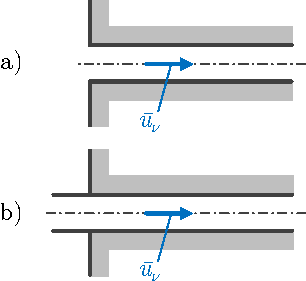
\includegraphics[width=0.8\textwidth]{images/rohr-geometrieverlust-eintritt.pdf}
            \end{minipage}%
            \\ \vspace{1mm}
            \rule{\dimexpr\cellwidth-2\TileSep}{0.5pt} \\ \vspace{0.5mm}
            \titlerm{Austritt}\\ \vspace{-0.5mm}
            \begin{minipage}{0.55\cellwidth-\TileSep}
                \centering
                \vspace{-4.5mm}
                \begin{align*}
                    \text{{\color{Bittersweet}Turbulent}: }\zeta_\text{a} &\approx \text{1,0} \\[-0.5ex]
                    \text{{\color{NavyBlue}Laminar}: }\zeta_\text{a}      &\approx \text{2,0}
                \end{align*}
            \end{minipage}%
            \begin{minipage}{0.45\cellwidth-\TileSep}
                \centering
                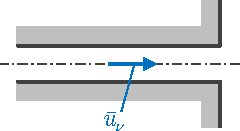
\includegraphics[width=0.66\textwidth]{images/rohr-geometrieverlust-austritt.pdf}
            \end{minipage}
        }{0}{1}{0}{0}

    % B5) Zweite Kachel rechts anbauen
    \setlength{\cellwidth}{100mm}
    \Tile{B5}{(A5.north east)}{\cellwidth}{\rowheight}
        {
            \vspace{-\TileSep}
            \titlerm{Schieber}\\ \vspace{2mm}
            \resizebox{\cellwidth-2\TileSep}{!}{%
            \begin{tabular}{c|c|c|c|c|c|c|c|c}
                \xrowht[()]{2.6mm} $\frac{s}{D}$          & \sfrac{1}{8} & \sfrac{2}{8} & \sfrac{3}{8} & \sfrac{4}{8} & \sfrac{5}{8} & \sfrac{6}{8} & \sfrac{7}{8} & \sfrac{8}{8} \\ \hline
                \xrowht[()]{2.6mm} $\frac{A_\text{s}}{A}$ & 0,948 & 0,856 & 0,743 & 0,609 & 0,466 & 0,315 & 0,159 & 0 \\ \hline
                \xrowht[()]{2.6mm} $\zeta_\text{s}$       & 0,07  & 0,26  & 0,81  & 2,06  & 5,52  & 17,0  & 97,8  &
            \end{tabular}
            }
            \\ \vspace{2mm}
            \begin{minipage}{0.4\cellwidth-\TileSep}
                \centering
                \begin{equation*}
                    \overline{u}_\nu = \frac{Q}{A_\nu}
                \end{equation*}
            \end{minipage}%
            \begin{minipage}{0.4\cellwidth-\TileSep}
                \centering
                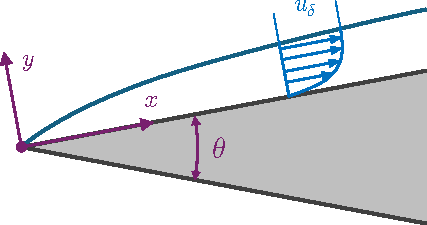
\includegraphics[width=0.8\textwidth]{images/keil.pdf}
            \end{minipage}
        }{0}{0}{0}{0}

\end{tikzpicture}